\documentclass[9pt,letterpaper,onecolumn]{rho-class/rho}
\usepackage[spanish,es-nodecimaldot,es-noindentfirst]{babel}
\usepackage{graphicx}
\usepackage{float}
\setlength{\parindent}{0pt}  % Elimina la sangría
\usepackage[utf8]{inputenc}
\usepackage[T1]{fontenc}
\setbool{rho-abstract}{true} % Set false to hide the abstract
\setbool{corres-info}{true} % Set false to hide the corresponding author section
\addbibresource{rho.bib}

% Definir el nuevo comando
\newcommand{\loopweb}{LoopWe$\mathbb{\flat}$ }

%----------------------------------------------------------
% TITLE
%----------------------------------------------------------

%\journalname{Example Template}
\title{\loopweb: Una red social en tu terminal}

%----------------------------------------------------------
% AUTHORS AND AFFILIATIONS
%----------------------------------------------------------
\author[$\dagger$]{Constanza Araya}
\author[$\dagger$]{Rodolfo Cifuentes}
\author[$\dagger$]{Bruno Martinez}
\author[$\dagger$]{Milton Hernández}
\author[$\dagger$]{Guliana Ruiz}

%----------------------------------------------------------

%\affil[1]{Affiliation of author one}
%\affil[2]{Affiliation of author two}
%\affil[3]{Affiliation of author three}
\affil[$\dagger$]{Universidad de Magallanes}

%----------------------------------------------------------
% DATES
%----------------------------------------------------------

\dates{Este informe fue compilado el \today}

%----------------------------------------------------------
% FOOTER INFORMATION
%----------------------------------------------------------

%\leadauthor{Author last name et al.}
%\footinfo{Creative Commons CC BY 4.0}
\smalltitle{Estructuras de datos}
%\institution{College name}
\theday{\today} %\today

%----------------------------------------------------------
% ARTICLE INFORMATION
%----------------------------------------------------------

%\corres{Provide the corresponding author information and publisher here.}
%\email{example@organization.com.}
%\doi{\url{https://www.doi.org/exampledoi/XXXXXXXXXX}}

%\received{March 20, 2024}
%\revised{April 16, 2024}
%\accepted{April 20, 2024}
%\published{May 21, 2024}

%\license{Rho LaTeX Class \ccLogo\ This document is licensed under Creative Commons CC BY 4.0.}

%----------------------------------------------------------
% ABSTRACT
%----------------------------------------------------------

\begin{abstract}
    \loopweb es una simulación en terminal de una red social, creada con el propósito de desarrollar habilidades en el manejo de volúmenes de datos mediante el uso de estructuras como Tablas hash, Listas enlazadas simples y Grafos.
\end{abstract}

%----------------------------------------------------------

\keywords{\loopweb, Simulación, Estructuras de datos, Tablas hash, Lista enlazada, Grafo}

%----------------------------------------------------------
\begin{document}
\maketitle
\tableofcontents
\newpage
\section{Introducción}
\loopweb es un proyecto diseñado para emular una red social enfocada en la música, desarrollado como una herramienta de aprendizaje práctico en el ámbito de estructuras de datos. Este sistema tiene como objetivo principal implementar y combinar estructuras como grafos, tablas hash y listas enlazadas logrando una solución funcional y adaptativa.

Mediante este desarrollo, se busca consolidar los conocimientos adquiridos a través de la creación de un entorno digital que imita las dinámicas de interacción y conexión propias de las redes sociales modernas.

Entre las funcionalidades implementadas, destacan la gestión de usuarios, gustos y comentarios y la recomendación de conexiones mediante la priorización de contenidos, demostrando la aplicabilidad de conceptos teóricos en un entorno práctico y estructurado.

\section{Objetivos}
El proyecto \loopweb se desarrolló con los siguientes objetivos específicos:

\begin{enumerate}
    \item Diseñar e implementar una simulación funcional de una red social que permita la gestión de perfiles de usuarios, la creación de conexiones entre ellos y la publicación de contenido.
    \item Integrar estructuras de datos complejas, como grafos y tablas hash, en un sistema cohesionado y escalable.
    \item Implementar algoritmos eficientes para optimizar las operaciones del sistema, tales como la recomendación de amigos basándose en afinidades o el ordenamiento de listas para una impresión ordenada por pantalla.
\end{enumerate}

\newpage
\section{Planificación del Proyecto}
La planificación del proyecto se llevó a cabo en varias etapas. En primer lugar, se definieron los objetivos generales del sistema y se exploraron las ideas fundamentales que darán forma al proyecto.

Centralmente se tienen tres ramas principales que se pueden observar en la figura \ref{fig:diagrama1}.
\begin{figure}[H]
    \centering
    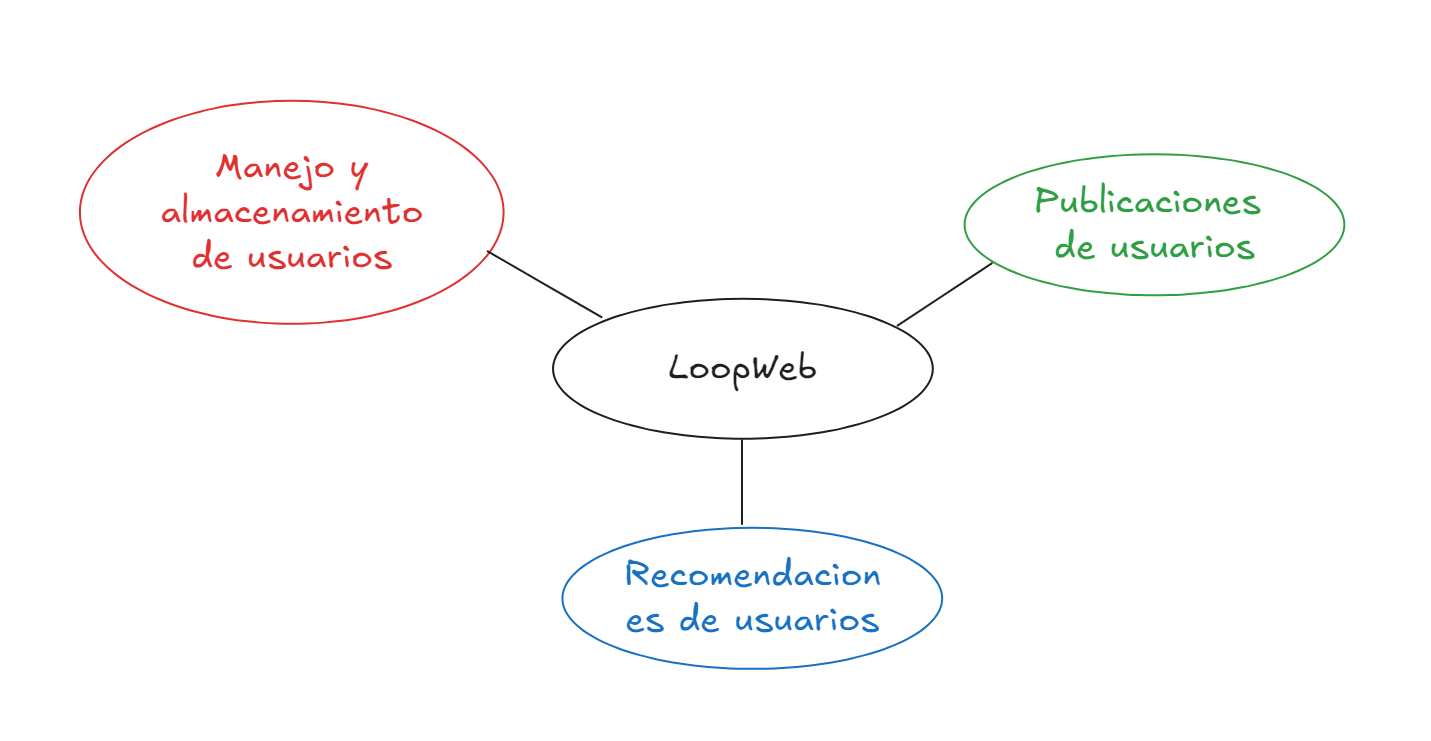
\includegraphics[width=0.5\textwidth]{./src/images/Diagrama1.png}
    \caption{Ejes principales de \loopweb}
    \label{fig:diagrama1}
\end{figure}

A continuación, se presentan los elementos clave que fueron considerados durante esta etapa de planificación:
\begin{enumerate}
    \item \textbf{Creación de perfiles de usuario:} Se busca implementar un sistema básico de perfil de usuario que permite a cada persona en la red social tener una representación digital que contiene:
    \begin{itemize}
        \item Nombre de usuario
        \item Edad del usuario
        \item Nacionalidad del usuario
        \item Géneros musicales que le gustan al usuario
        \item Bandas o artistas que le gustan al usuario (tratadas solo como bandas dentro del programa)
        \item Comentarios que ha realizado el usuario
        \item Amistades del usuario con otros perfiles de la red
    \end{itemize}
    \item \textbf{Establecimiento de conexiones entre usuarios:} Continuando con el punto anterior se busca desarrollar una funcionalidad que permita a los usuarios establecer relaciones de amistad, simulando un comportamiento cercano al de una red social.
    \item \textbf{Publicación y visualización de publicaciones:} Los usuarios podrán crear publicaciones y ver aquellas que estén relacionadas con sus gustos musicales, lo que ``fomentará la interacción'' dentro de la red social.
    \item \textbf{Exploración y recomendación de usuarios:} Este programa permitirá a los usuarios explorar otros perfiles recomendados para ellos (recomendaciones que se basarán en la cercanía de edad y los gustos musicales), lo anterior permitirá promover una experiencia personalizada para cada usuario.
    \item \textbf{Realización de búsquedas eficientes:} Se implementarán algoritmos de búsqueda basados en grafos para permitir la localización eficiente de usuarios dentro de la red social, optimizando la experiencia de navegación.
    \item \textbf{Eficiencia y Escalabilidad:} El sistema será diseñado utilizando estructuras de datos como tablas hash y listas enlazadas, lo que garantiza un rendimiento óptimo incluso con grandes volúmenes de datos.
    \item \textbf{Opción Administrativa:} Se plantea una opción de administración que permitirá gestionar de manera sencilla los usuarios, gustos y sus publicaciones, facilitando el control dentro de la red social así como la creación de nuevos usuarios.
\end{enumerate}

Para una correcta realización del proyecto se crean tres diagramas de flujo que juntos describen el comportamiento esperado de la aplicación.

En la figura \ref{fig:diagrama2} se muestra el diagrama de flujo principal de \loopweb, que se divide en dos partes: un modo de administración (figura \ref{fig:diagrama3}) y otro para la interacción de un usuario en particular (figura \ref{fig:diagrama4}).
\begin{figure}[!h]
    \centering
    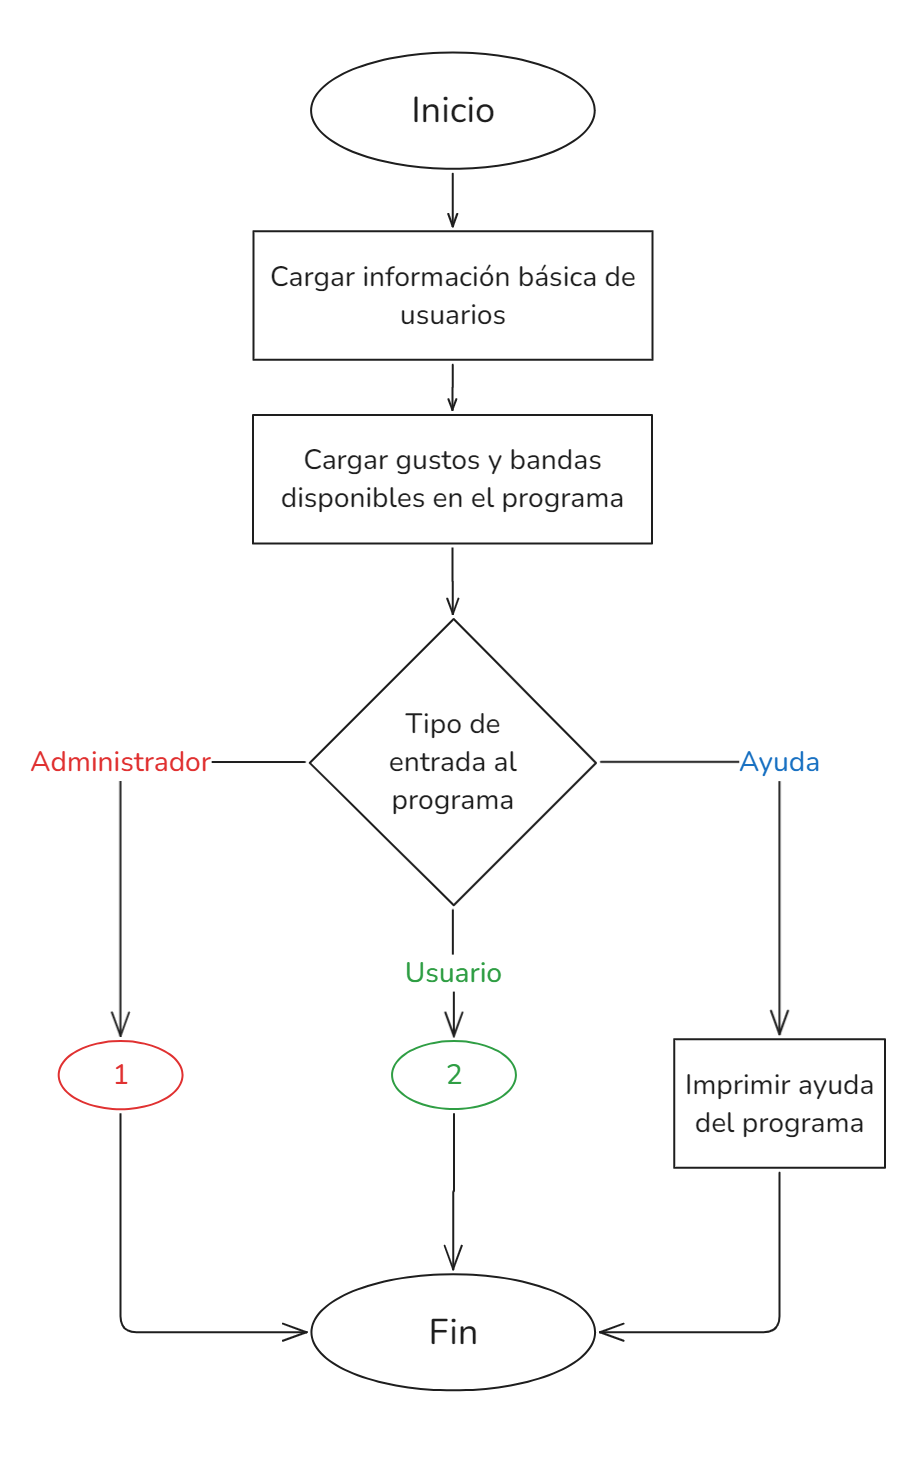
\includegraphics[width=0.3\textwidth]{./src/images/Diagrama2.png}
    \caption{Diagrama de flujo prinicpal de \loopweb}
    \label{fig:diagrama2}
\end{figure}

\begin{figure}[!h]
    \centering
    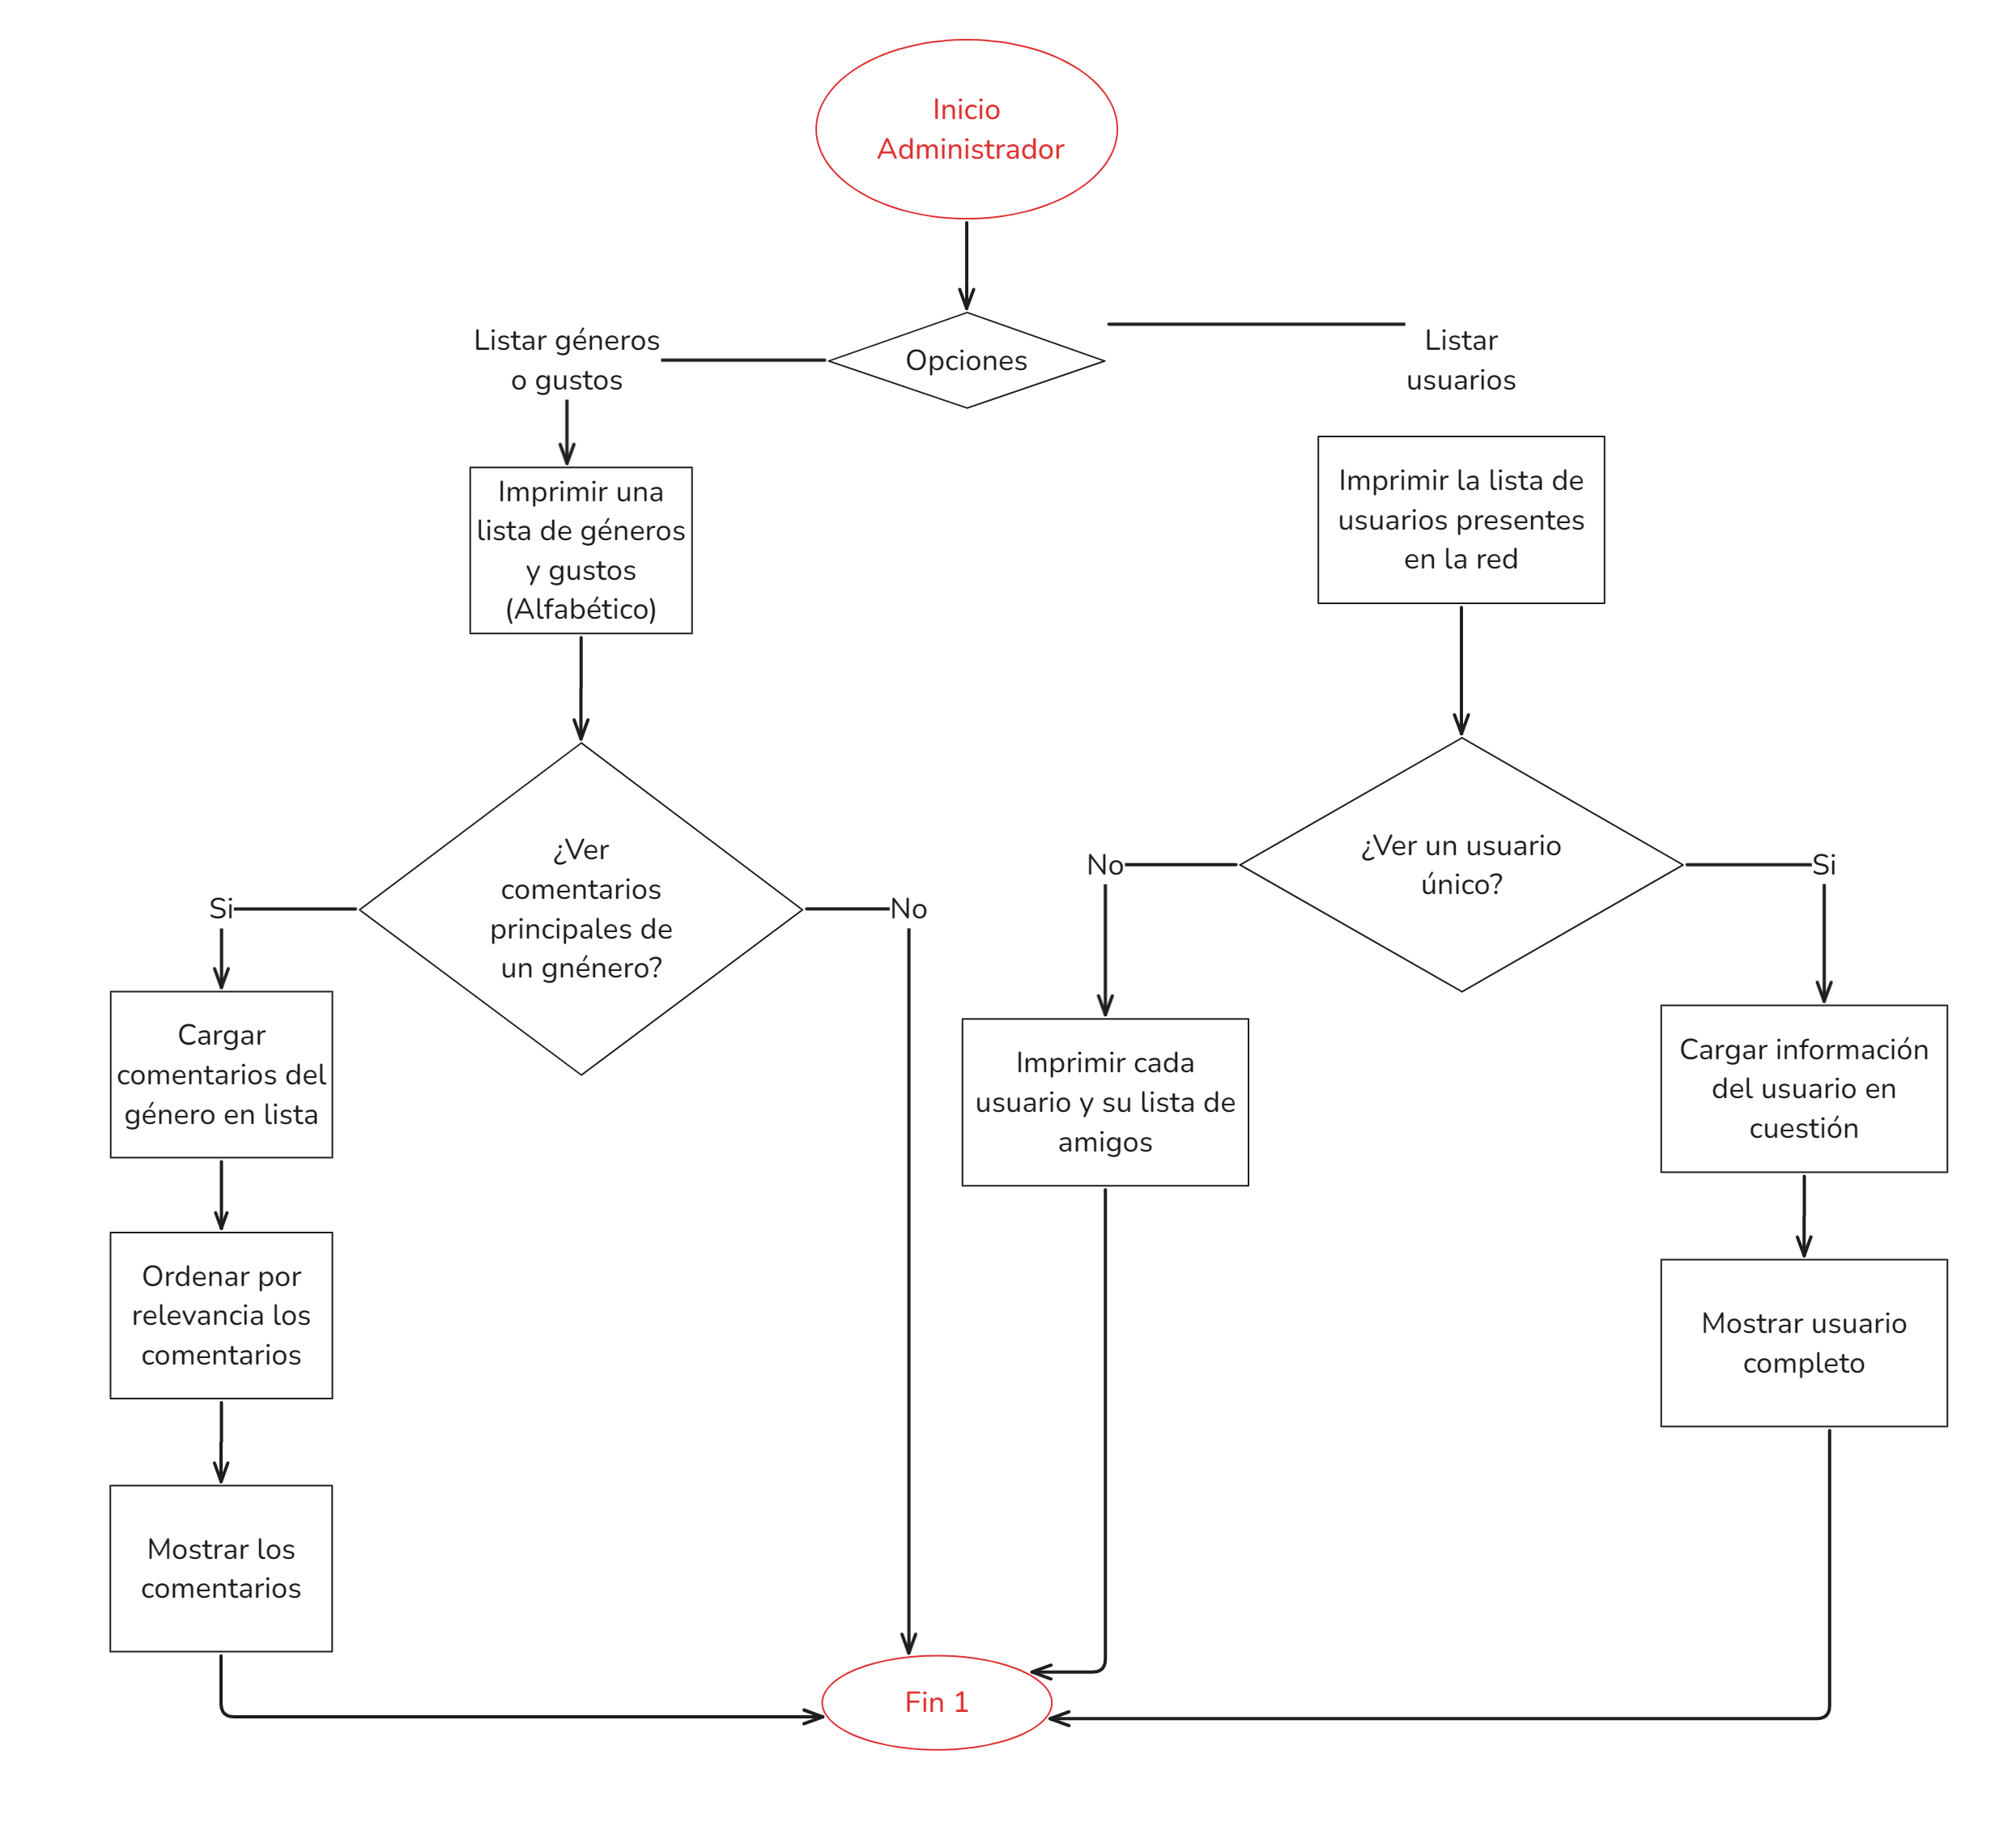
\includegraphics[width=0.5\textwidth]{./src/images/Diagrama3.png}
    \caption{Flujo de un administrador de \loopweb}
    \label{fig:diagrama3}
\end{figure}

\begin{figure}[p]
    \centering
    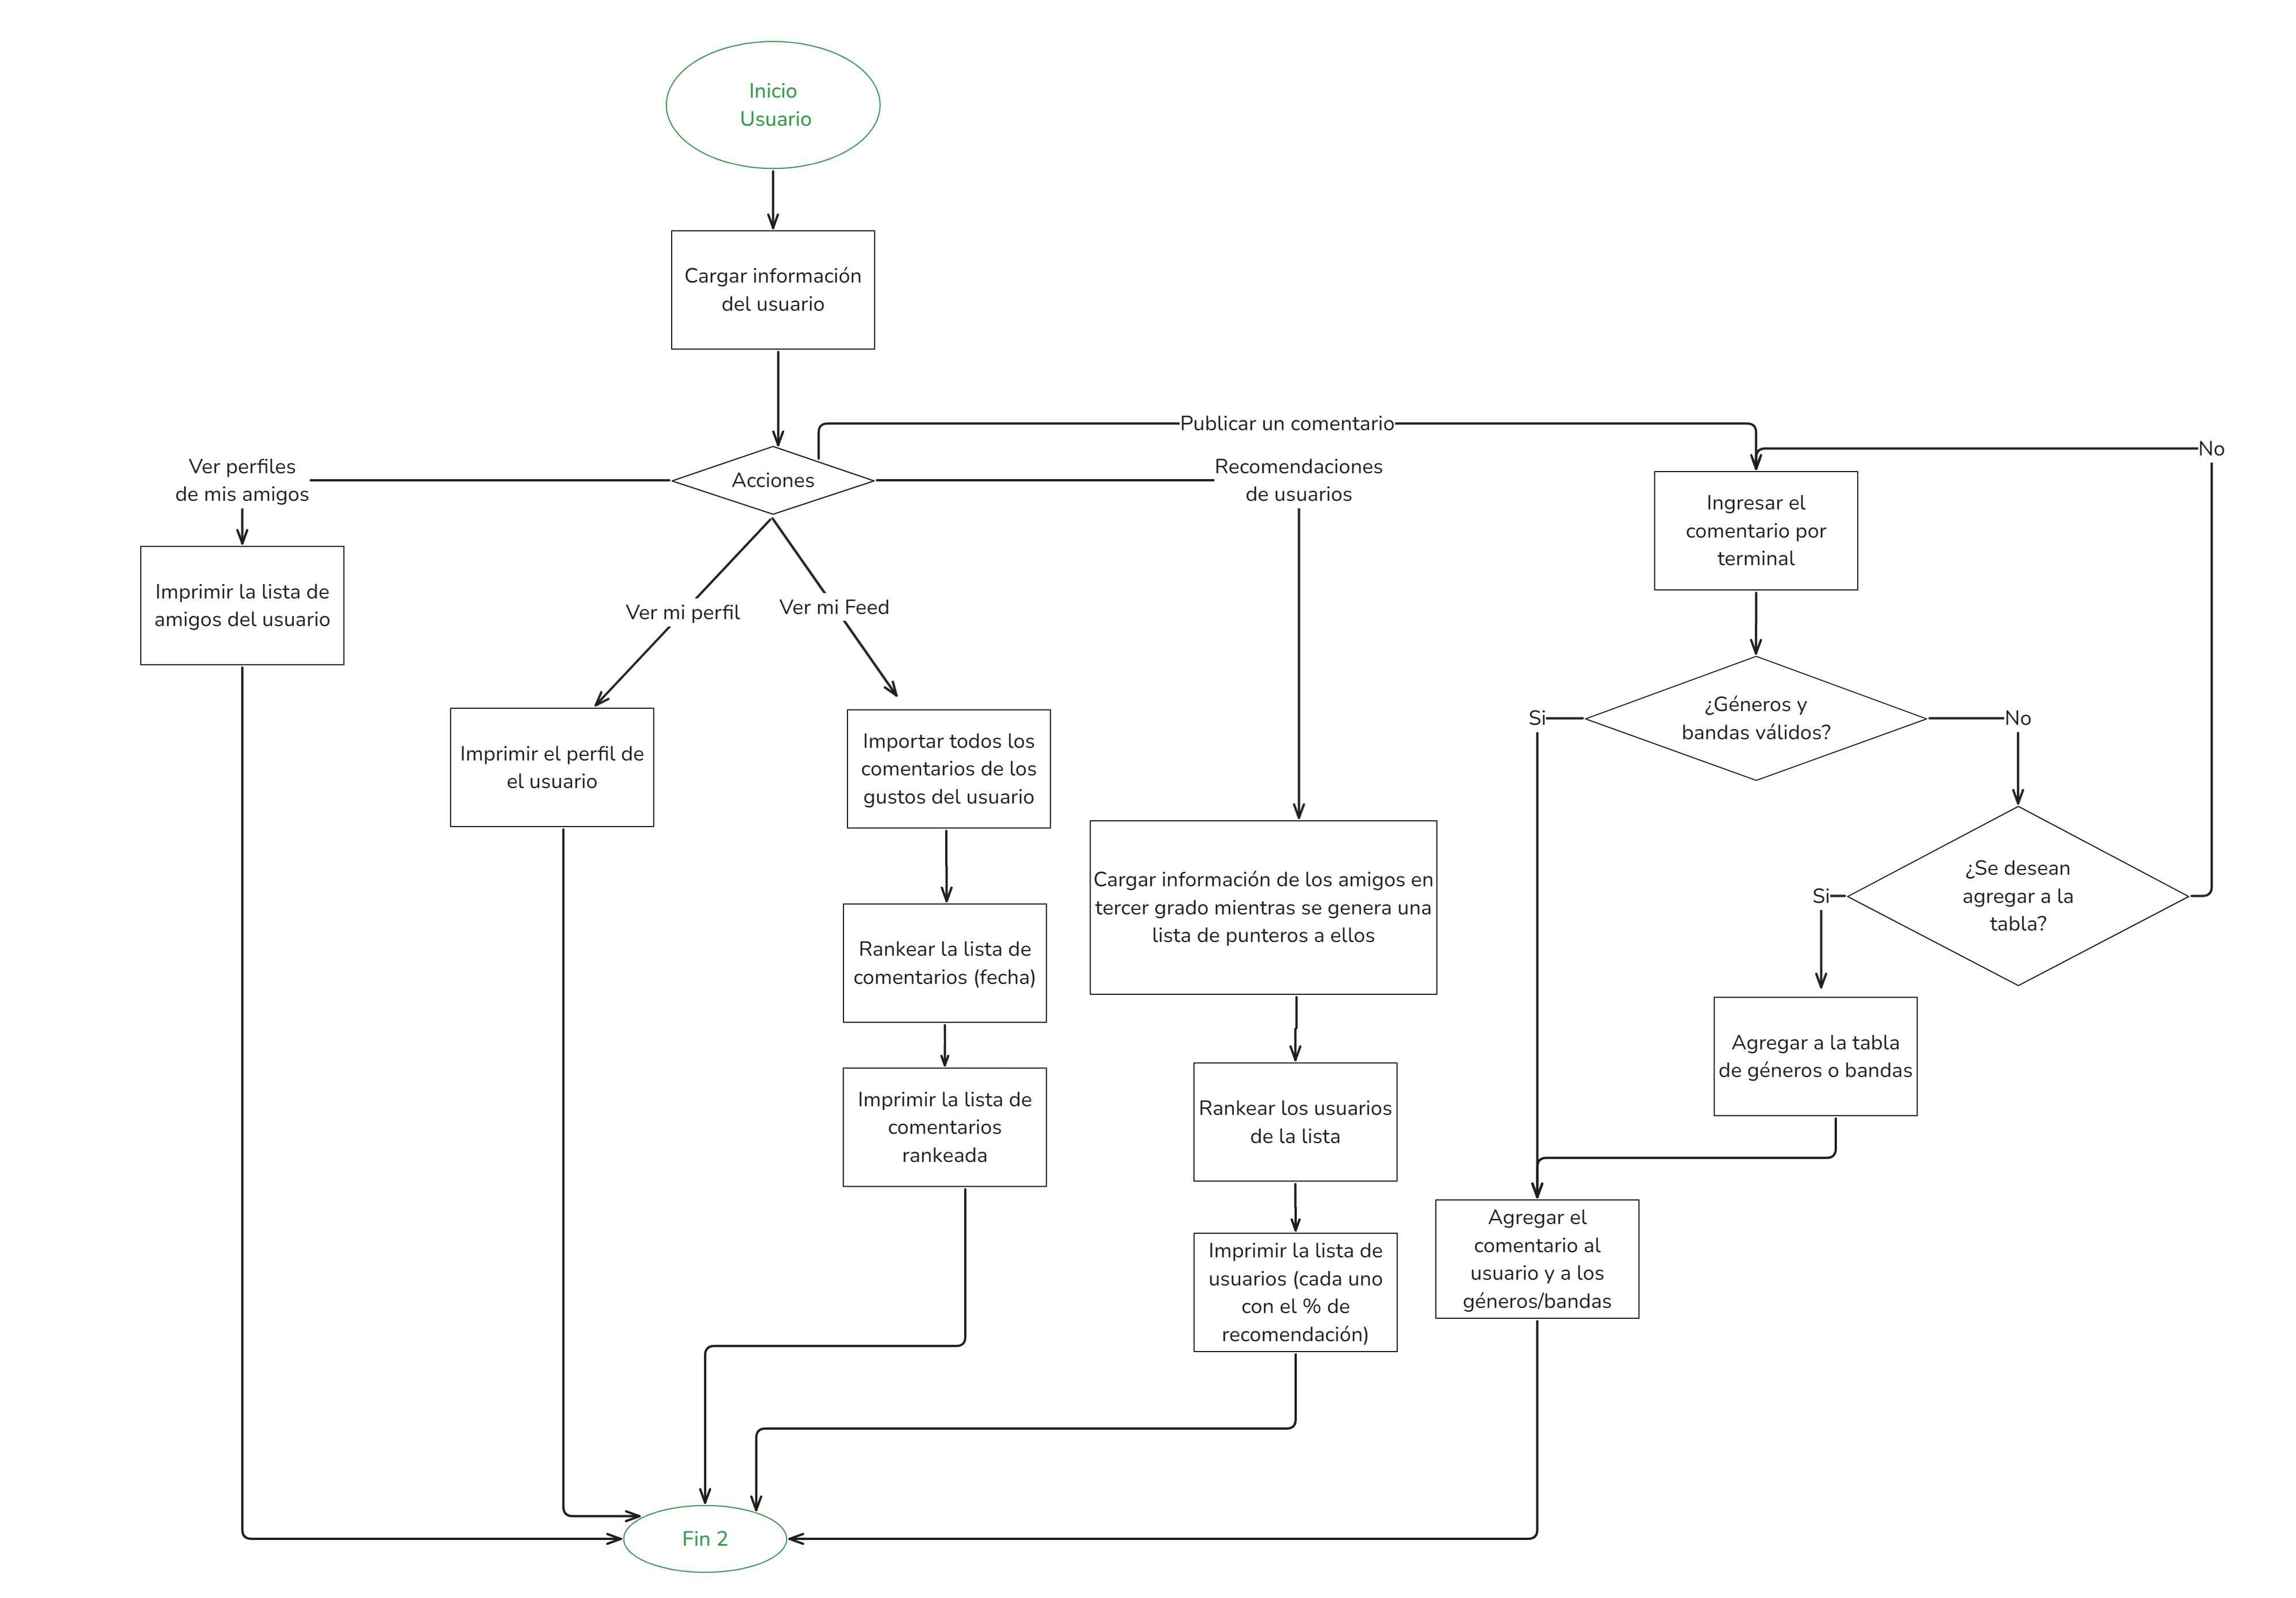
\includegraphics[width=1\textwidth]{./src/images/Diagrama4.png}
    \caption{Flujo de un usuario de \loopweb}
    \label{fig:diagrama4}
\end{figure}


\newpage
\input{src/sections/investigación.tex}
\newpage
\section{Estructuras de datos implementadas}
Dentro de \loopweb se utilizaron en esencia dos estructuras de datos: Tablas hash y Listas enlazadas simples. Ambas tienen sus propias características y usos específicos, y se han diseñado para cumplir con diferentes objetivos propuestos para la aplicación.

%-----------------------------%
\subsection{Tablas Hash}
El uso de esta estructura de datos se debe a su eficiencia a la hora de almacenar información. Esta estructura fue utilizada para almacenar los \textbf{Usuarios}, \textbf{Bandas}, \textbf{Generos} y \textbf{Comentarios} que existen dentro de la ``base de datos'' de \loopweb.

Las tablas hash también son fáciles de crear y eliminar en forma recursiva y los datos que se guardan en ellas pueden ser de cualquier tipo, lo que facilita la gestión de información de los usuarios o bandas quienes no tienen necesariamente un Identificador numérico.

%-----------------------------%
\subsection{Listas Enlazadas Simples}
Esta estructura es el `Engranaje central' de este programa, escogida por su gran flexibilidad en cuanto a espacio.

El principal uso de esta estructura de datos se encuentra en la creación de ``Enlaces a las tablas hash'' anteriores. Esto permite el almacenamiento de información que se encuentra en las tablas sin necesidad de duplicar la información presente en las mismas.

%-----------------------------%
\subsection{Grafos}
El almacenamiento de usuarios es la caracteristica fundamental de \loopweb, esencial para su correcto funcionamiento.

Para ``dar vida'' a esta estructura de datos dentro del programa no se creó una estructura de datos especifica sino que se usó una abstracción de los conceptos de grafos mediante las tablas hash.

Los algoritmos para grafos fueron utilizados para recorrer las conexiones de los usuarios y poder recomendar amigos entre amigos de amigos para ello se usó el algoritmo \textbf{BFS} para recorrer el grafo de usuarios.

%-----------------------------%
\subsection*{¿Qué otras estructuras de datos podrían haber sido implementadas?}
El uso de Listas enlazadas simples permite la facilidad de implementación de todas las funciones propias de \loopweb, sin embargo estructuras como las Listas Doblemente Enlazadas o las Colas podrían dar más eficiencia a ciertas operaciones.

\newpage
\section{En busca de la eficiencia}
\subsection{Algoritmos de ordenamiento}
Los \textbf{algoritmos de ordenación} son un conjunto de instrucciones que toman un arreglo o lista como entrada y organizan los elementos en un orden particular.
Las ordenaciones suelen ser numéricas o una forma de orden alfabético (o lexicográfico), y pueden ser en orden ascendente (AZ, 0$-$9) o descendente (ZA, 9$-$0).

Estos algoritmos son fundamentales dado que permiten reducir la tarea de ordenar datos a una tarea más simple y eficiente. Estos algoritmos tienen aplicaciones directas en algoritmos de búsqueda, algoritmos de bases de datos, algoritmos de estructura de datos y muchos más.

Para la creación de este programa se requiere la ordenación de diferentes listas enlazadas (Listas de usuarios, de bandas, de géneros y comentarios) bajo criterios tanto numéricos como lexicográficos.

Inicialmente se planteó el uso del algoritmo Bubble Sort o \textbf{Ordenamiento por intercambio} el cuál, compara pares de elementos adyacentes y los intercambia si están en el orden incorrecto. Repite este proceso hasta que todos los elementos estén ordenados. Este algoritmo es fácil de implementar pero su eficiencia es bastante baja, con una complejidad temporal de $O(n^2)$. Dado que su rendimiento empeora conforme crece el tamaño de la lista, se consideró que no era adecuado para este proyecto, donde se manejan conjuntos de datos más grandes.
\begin{figure}[H]
    \centering
    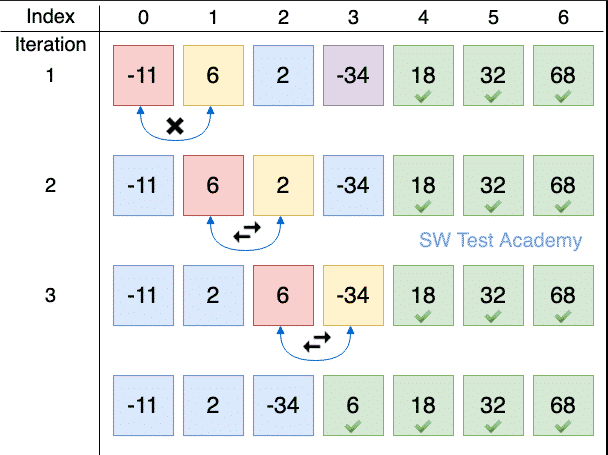
\includegraphics[width=0.5\textwidth]{./src/images/BubbleSort.png}
    \caption{Bubble Sort}
    \label{fig:BubbleSort}
\end{figure}
\newpage
Por otro lado el algoritmo Merge Sort o \textbf{Ordenamiento por Mezcla} divide el conjunto de elementos en subconjuntos más pequeños, los ordena por separado y luego los fusiona para obtener un conjunto ordenado más grande. Este algoritmo utiliza la estrategia de ``divide y vencerás'', lo que le da una eficiencia mucho mayor que Bubble Sort, con una complejidad temporal de $O(n \log n)$. Dado que el proyecto implicaba manejar (posiblemente) grandes volúmenes de datos, se optó por Merge Sort debido a su mejor comportamiento en términos de rendimiento.
\begin{figure}[H]
    \centering
    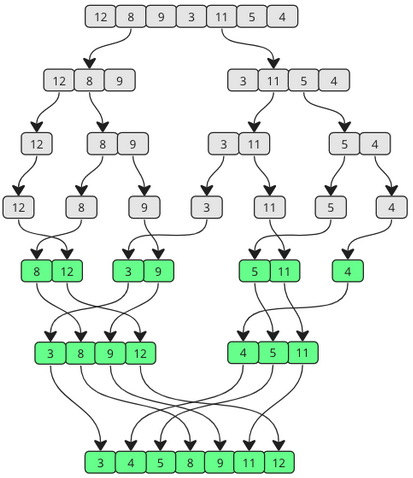
\includegraphics[width=0.5\textwidth]{./src/images/MergeSort.png}
    \caption{Merge Sort}
    \label{fig:MergeSort}
\end{figure}
\newpage
\subsection{JSON}
\textbf{JSON} es un formato de intercambio de datos utilizados para almacenar e intercambiar información estructurada de manera legible. Es ampliamente usado para la transferencia de datos entre servidores y clientes.
\subsubsection*{¿Para qué se utiliza un archivo JSON?} % Esto sería un subtítulo
\textbf{JSON} almacena información en forma de pares clave-valor y es utilizado principalmente para transferir datos estructurados. Un archivo JSON puede contener diferentes tipos de datos, como cadenas de texto, números, objetos, arreglos, valores booleanos y null, como se muestra en la figura \ref{fig:json}
\begin{figure}[H]
    \centering % Para que aparezca centrada
    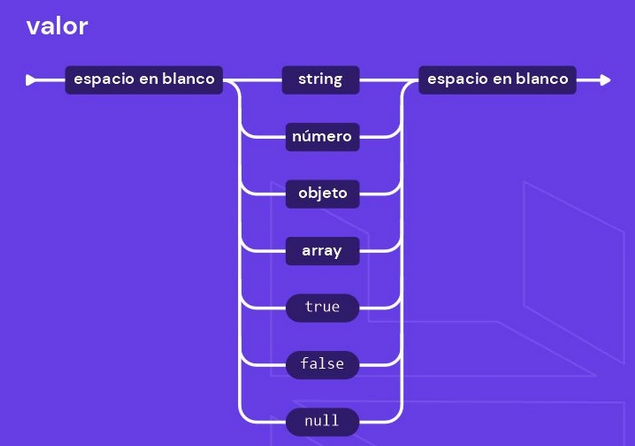
\includegraphics[width=0.5\textwidth]{./src/images/json.png} % Esta linea incluye la imagen
    \caption{Diagrama json} % Este es el mensaje que acompaña la imagen
    \label{fig:json} % Esta es la referencia a la imagen
\end{figure}
En el estracto de código \ref{lst:json} se muestra un ejemplo de un archivo JSON que contiene información sobre un usuario perteneciente a \loopweb
\begin{lstlisting}[language=C, caption={Ejemplo de .json}, label={lst:json}]
{
  "userName": "Alice",
  "age": 18,
  "nationality": "Spain",
  "genres": [ "rock", "pop" ],
  "artists": [ "rihanna", "ladyGaga" ],
  "description": "Amante de los festivales de musica.",
  "friends": [ "Bob", "Carol", "Mallory" ]
}
\end{lstlisting}

\newpage
\subsubsection*{¿Cómo utilizar JSON en C?}
Para trabajar con archivos .json en C, es necesario utilizar librerías externas. Algunas opciones son:
\begin{enumerate}
    \item Jansson
    \item Json-c
    \item cjson
\end{enumerate}
En este caso, se usará la librería \href{https://github.com/akheron/jansson}{Jansson}.

Jansson es una librería de C para trabajar con datos JSON, simple, sin dependencias externas y con documentación completa.

Algunas de las funcionalidades más importantes de Jansson son:
\begin{enumerate}
    \item \textbf{json\_error\_t}: Tipo de dato para almacenar errores durante la lectura de un archivo JSON.
    \begin{lstlisting}[language=C, caption={json\_error\_t}]
        json_error_t error;
    \end{lstlisting}
    \item \textbf{json\_t}: Tupo de dato para unobjeto JSON, siempre a través de un puntero.
    \begin{lstlisting}[language=C, caption={json\_t}]
        json_t *materias_json = json_object_get(alumnos_json,"materias");
    \end{lstlisting}
    \item \textbf{json\_loadf()}: Carga el contenido de un archivo JSON en una variable de tipo json\_t.
    \begin{lstlisting}[language=C, caption={json\_loadf}]
        json_t *json = json_loadf(archivo,0,&error);
    \end{lstlisting}
    \item \textbf{json\_object\_get()}: Accede a los valores de un objeto JSON.
    \begin{lstlisting}[language=C, caption={json\_object\_get}]
        json_object_value(alumnos_json,"nombre");
    \end{lstlisting}
    \item \textbf{json\_string\_value()}: Extrae el valor de una cadena de texto en JSON.
    \begin{lstlisting}[language=C, caption={json\_string\_value}]
        json_string_value(json_object_value(alumnos_json,"nombre"));
    \end{lstlisting}
    \newpage
    \item \textbf{json\_integer\_value()}: Extrae el valor de un entero de un objeto JSON.
    \begin{lstlisting}[language=C, caption={json\_integer\_value}]
        json_integer_value(json_object_value(alumnos_json,"edad"));
    \end{lstlisting}
\end{enumerate}

La utilización de arhcivos JSON para el almacenamiento de la información de este programa es crucial para que la información sea sencilla de almacenar y eficiente de leer, permitiendo no cargar toda la información del programa en cada acción sino cargar \textbf{solo lo necesario} en| cada momento.
\newpage
\section{Algunos algoritmos y funciones destacables}
A continuación se explican algunas de las funciones más interesantes que se construyeron durante el desarrollo del programa.
%----------------------------%
\subsection{Funcion GetOPT}

\textbf{getOPT} es una función parte de las librerías estándar de C que permite una cómoda interacción con la línea de comandos facilitando el uso de banderas de opciones.

Esta función recibe como argumento un string de texto y devuelve un entero que representa el código de acceso con el que se quiere ingresar.

A pesar de que esta funcionalidad que es de por sí bastante útil se optó por el uso de la función \textbf{getoptLong()} para poder utilizar banderas más extensas. Así dentro de \loopweb se pueden ocupar las opciones \texttt{./build/loopweb.out -h},  \texttt{./build/loopweb.out -a}, \texttt{./build/loopweb.out -u <nombre>}, \texttt{./build/loopweb.out ----help}, \texttt{./build/loopweb.out ----administrador} ó \texttt{./build/loopweb.out ----user <nombre>}.


%----------------------------%
\subsection{Implementacion de mergeSort para Listas enlazadas}
El algoritmo de ordenamiento de merge sort es utilizado principalmente sobre arreglos de datos, pero también puede ser utilizado sobre listas enlazadas. En el presente proyecto se implementó una triada de funciones que juntas permiten implementar merge sort sobre listas enlazadas (A continuación se muestra un ejemplo con listas de enlaces a géneros, aunque se puede implementar con cualquier lista enlazada simple):
\begin{enumerate}
    \item \textbf{split\_genreLinkList}: Esta función divide una lista enlazada en dos mitades, parte importante y esencial para el merge sort.
    \begin{lstlisting}[language=C, caption={split\_genreLinkList}, label={lst:codigo}]
/**
* @brief Divide una lista enlazada en dos mitades.
* @param source Puntero al nodo inicial de la lista a dividir.
* @param frontRef Referencia a la primera mitad de la lista.
* @param backRef Referencia a la segunda mitad de la lista.
*/
void split_genreLinkList(GenreLinkPosition source, GenreLinkPosition* frontRef, GenreLinkPosition* backRef)
{
    GenreLinkPosition slow, fast;
    slow = source;
    fast = source->next;
    while (fast != NULL) {
        fast = fast->next;
        if (fast != NULL) {
            slow = slow->next;
            fast = fast->next;
        }
    }
    *frontRef = source;
    *backRef = slow->next;
    slow->next = NULL;
}
\end{lstlisting}
    \item \textbf{merge\_genreLinkLists:} Esta función fusiona dos listas enlazadas ordenadas en una sola lista ordenada.
\begin{lstlisting}[language=C, caption={fusion de listas}, label={lst:codigo}]
/**
* @brief Fusiona dos listas enlazadas ordenadas en una sola lista ordenada
* @param a Puntero a la primera lista ordenada
* @param b Puntero a la segunda lista ordenada
* @return Puntero al nodo inicial de la lista fusionada ordenada
*/
GenreLinkPosition merge_genreLinkLists(GenreLinkPosition a, GenreLinkPosition b)
{
    if (a == NULL) return b;
    if (b == NULL) return a;
    GenreLinkPosition result;
    if (strcmp(a->genre, b->genre) <= 0) {
        result = a;
        result->next = merge_genreLinkLists(a->next, b);
    } else {
        result = b;
        result->next = merge_genreLinkLists(a, b->next);
    }
    return result;
}
\end{lstlisting}
    \item \textbf{mergerSort\_genreLinkList}: Esta función controla el algoritmo como tal llamando \textbf{recursivamente} a las funciones anteriores y a sí misma.
\begin{lstlisting}[language=C, caption={mergerSort\_genreLinkList}, label={lst:codigo}]
/**
* @brief Ordena una lista enlazada utilizando el algoritmo merge sort.
* @param headRef Referencia al puntero del nodo inicial de la lista a ordenar.
*/
void mergeSort_genreLinkList(GenreLinkPosition* headRef)
{
    GenreLinkPosition head = *headRef;
    GenreLinkPosition a, b;
    if ((head == NULL) || (head->next == NULL)) {
        return;  /**<si la lista esta vacia o tiene un solo elemento, no hay que ordenar */
    }
    split_genreLinkList(head, &a, &b);
    mergeSort_genreLinkList(&a);  /**<ordena la primera mitad */
    mergeSort_genreLinkList(&b);  /**<ordena la segunda mitad */
    *headRef = merge_genreLinkLists(a, b);  /**<fusiona las dos mitades ordenadas */
}
\end{lstlisting}
\end{enumerate}

Estas funciones fueron implementadas y ligeramente modificadas al interior del código para ajustarse a cada uno de los casos de uso necesarios\footnote{Es importante notar que todas las funciones hacen uso de punteros a los nodos de la lista enlazada y que además la función principal debe recibir como parámetro un puntero al \textbf{Primer} nodo de la lista enlazada y NO al centinela de la misma}.


%----------------------------%
\newpage
\subsection{Algoritmo BFS para recorrido de un grafo}

El algoritmo BFS (algoritmo de búsqueda en profundidad) se encarga de recorrer los usuarios conectados por ``nivel'' y
es utilizado para generar las recomendaciones de amigos, esta información se guarda en una lista de usuarios visitados, esto se hace para evitar repetir usuarios que ya se han visitado anteriormente.

Las recomendaciones dentro del programa se restringen a los amigos en tercer grado (Los amigos de amigos de amigos) para evitar una lista muy larga de recomendaciones.

\begin{lstlisting}[language=C, caption={Pseudocodigo del algoritmo BFS}, label={lst:BFS}]
    BFS(Grafo G, Nodo inicial S):
    Crear una cola vacia Q
    Crear un conjunto vacio VISITADOS
    Crear un diccionario NIVELES, donde cada nodo tiene un nivel asociado

    Encolar S en Q
    Marcar S como visitado anhadiendolo a VISITADOS
    Asignar nivel 1 a S en NIVELES

    Mientras Q no este vacia:
        Nodo actual <- desencolar Q
        Procesar Nodo actual (EJ: Almacenarlo en una lista de recomendaciones)

        Para cada vecino V de Nodo actual en G:
            Si V no esta en VISITADOS:
                Encolar V en Q
                Marcar V como visitado anhadiendolo a VISITADOS
                Asignar nivel (NIVELES[Nodo actual] + 1) a V en NIVELES
\end{lstlisting}
\newpage
\section{Apariencia de loopweb}
La función \texttt{print\_loopweb} tiene como objetivo procesar y resaltar publicaciones desde una cadena de caracteres. Las palabras que comienzan con \texttt{@} (bandas o artistas) se imprimen en verde, mientras que las que comienzan con \texttt{\#} (géneros) se imprimen en rojo.

Esta función divide el texto en palabras, procesa cada una (carácter por carácter) y aplica los colores correspondientes a los géneros o bandas, asegurando que caracteres mal ubicados o repetidos no interfieran con el formato.

Un aspecto clave del funcionamiento es el uso de \texttt{strtok()} para dividir el texto en palabras y el ciclo que recorre cada carácter para identificar y resaltar correctamente los géneros y bandas. La línea \texttt{printf(ANSI\_COLOR\_GREEN);} es esencial, ya que aplica el color verde a las palabras que comienzan con \texttt{@}, permitiendo que se resalten correctamente en la salida (análogamente para los géneros).

El formato resultante permite identificar fácilmente los géneros (\texttt{@}) y bandas (\texttt{\#}) en las publicaciones, mejorando la visualización del contenido en \loopweb. Esta funcionalidad contribuye a resaltar elementos clave de manera clara y eficiente, y es útil para visualizar perfiles o contenido dinámico de los usuarios.

\section{Experiencia del Usuario}
En \loopweb, la experiencia del usuario ha sido diseñada para ser dinámica, llamativa y altamente interactiva, esto debido a su característica de ser una aplicación no estática (donde todas las acciones son realizadas por el usuario y no existe generación automática o programada de contenido).

Para poder llevar a cabo este dinamismo se hizo uso de los colores proporcionados por el código ANSI, que permite representar colores en la pantalla.
\newpage
\section{Conlusiones}
LoopWeb ha sido un proyecto que ha supuesto un gran reto en diversos sentidos para quienes lo desarrollaron, esto debido a su complejidad conceptual y la necesidad de llevar a cabo una correcta abstracción del problema para poder implementarlo en un entorno no tan gráfico como es el terminal.

La investigación fue un punto clave para el correcto desarrollo del programa, ya que permitió un correcto enfoque en aquellos puntos que se consideraron podrían ser de interés para un producto final, como la implementación de algoritmos de recomendación o las restricciones de longitud de las publicaciones.

El trabajo en equipo fue también un punto clave, logrando unir esfuerzos de diferentes profesores para conseguir una documentación completa y un código funcional y eficiente.
\newpage

\nocite{*}
\printbibliography[heading=bibintoc]

\end{document}